\documentclass[xetex,mathserif,serif]{beamer}
\usepackage{polyglossia}
\setdefaultlanguage[babelshorthands=true]{russian}
\usepackage{minted}
\usepackage{tabu}

\useoutertheme{infolines}

\usepackage{fontspec}
\setmainfont{FreeSans}
\newfontfamily{\russianfonttt}{FreeSans}

\tabulinesep=0.7mm

\title{Domain-Driven Design}
\author[Юрий Литвинов]{Юрий Литвинов \newline \textcolor{gray}{\small\texttt{yurii.litvinov@gmail.com}}}

\date{06.04.2018г}

\begin{document}
	
	\frame{\titlepage}

	\section{Введение}

	\begin{frame}
		\frametitle{Domain-Driven Design, напоминание}
		\begin{itemize}
			\item Архитектура приложения строится вокруг \textbf{Модели предметной области}
			\item Модель определяет \textbf{Единый язык}, на котором общаются и разработчики, и эксперты, описывая естественными фразами то, что происходит и в программе, и в реальности
			\item Модель --- это не только диаграммы, это ещё (и прежде всего) код, и устное общение
			\item Модель строится в процессе непрерывной \textbf{Переработки знаний}
			\begin{itemize}
				\item Рефакторинг --- неотъемлемая часть процесса
			\end{itemize}
		\end{itemize}
	\end{frame}

	\begin{frame}
		\frametitle{Книжка, по которой рассказ}
		\framesubtitle{И откуда картинки}
		Эрик Эванс, ``Предметно-ориентированное проектирование. Структуризация сложных программных систем''. М., ``Вильямс'', 2010, 448 стр.
		\begin{center}
			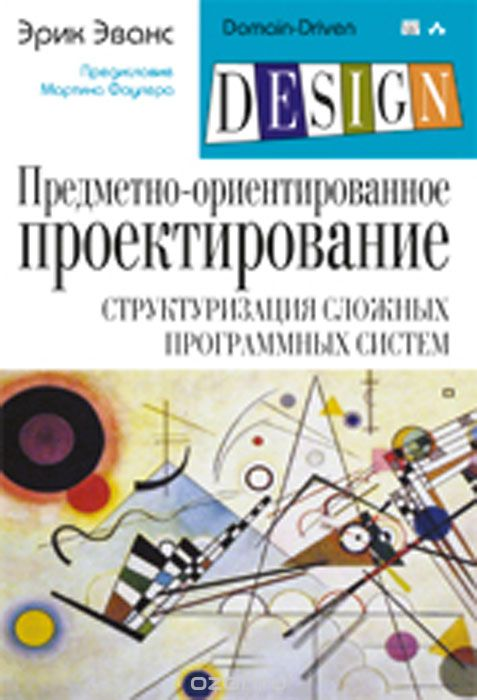
\includegraphics[width=0.25\textwidth]{dddCover.jpg}
		\end{center}
	\end{frame}

	\section{Единый язык}

	\begin{frame}
		\frametitle{Единый язык}
		\begin{itemize}
			\item У программистов и специалистов предметной области свой профессиональный жаргон
			\item Свои жаргоны появляются даже среди групп разработчиков в одном проекте
			\item Необходимость перевода размывает смысл понятий
			\item ``Еретики'' используют понятия в разных смыслах
			\item Единый язык --- понятия из модели (классы, методы), паттерны, элементы ``высокоуровневой'' структуры системы (которая не отражается в коде)
			\item Изменения в языке --- рефакторинг кода
			\item Языков в проекте может быть много
		\end{itemize}
	\end{frame}

	\begin{frame}
		\frametitle{Без единого языка}
		\begin{center}
			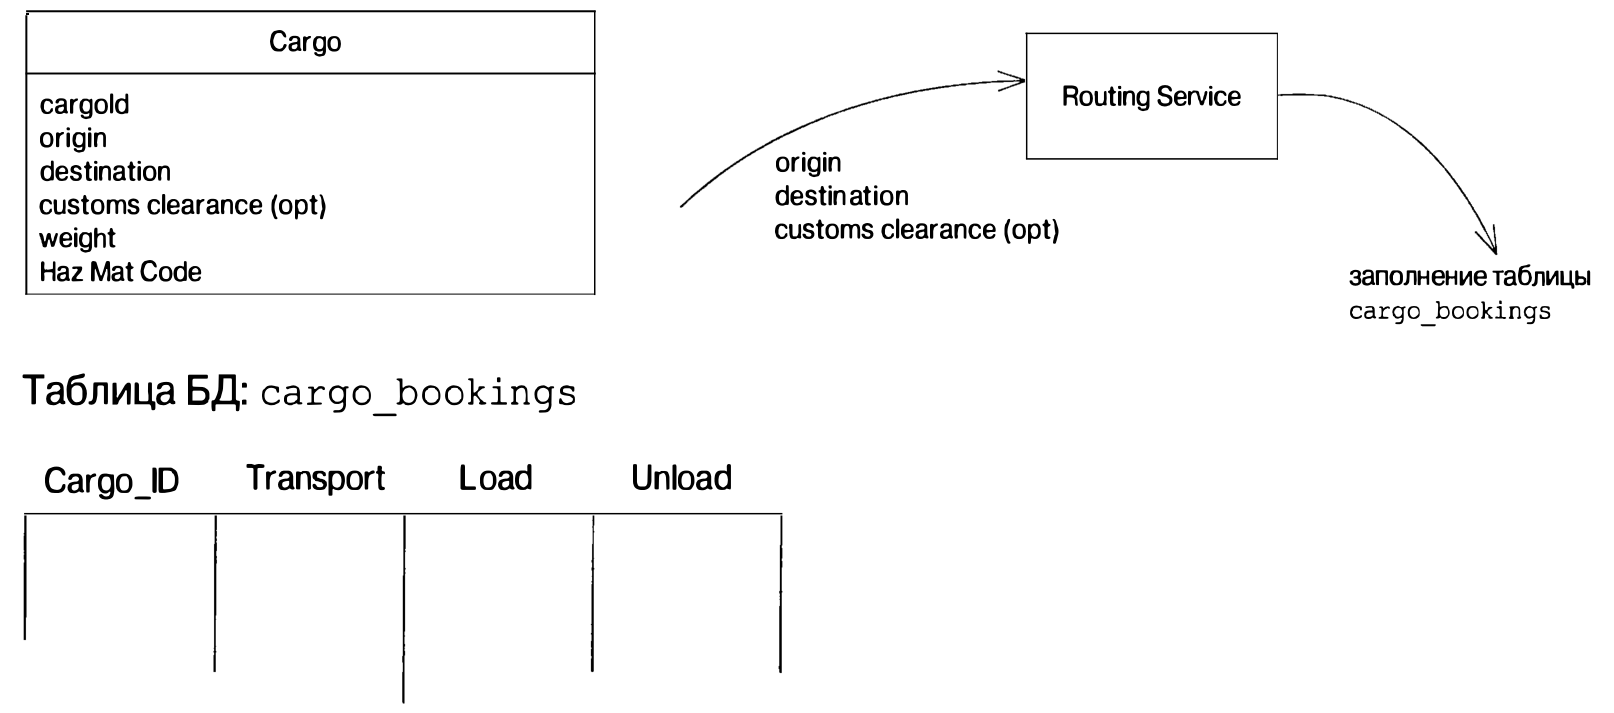
\includegraphics[height=0.6\textheight]{lowAbstractionLanguage.png}
		\end{center}
	\end{frame}

	\begin{frame}
		\frametitle{С единым языком}
		\begin{center}
			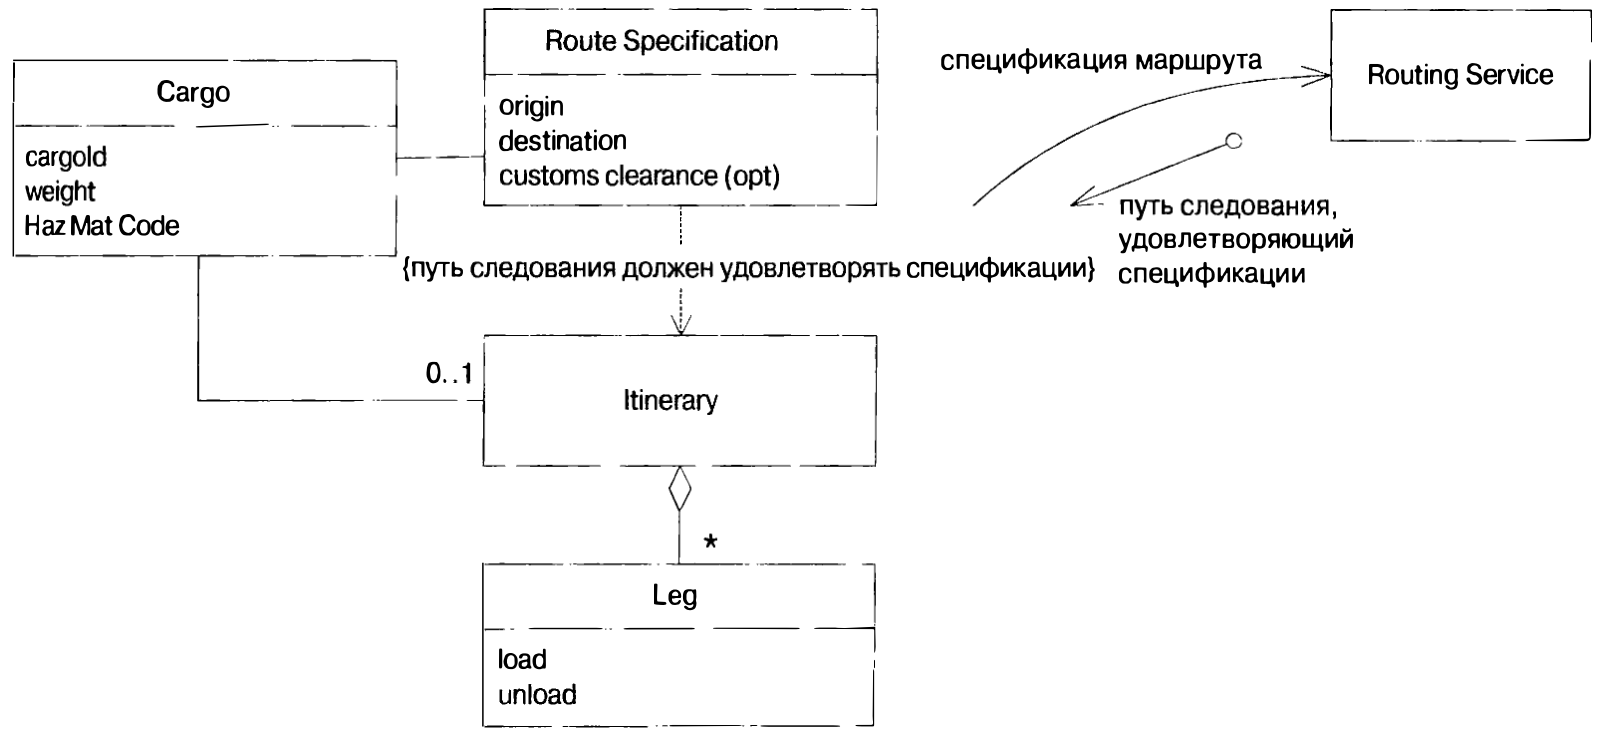
\includegraphics[height=0.6\textheight]{highAbstractionLanguage.png}
		\end{center}
	\end{frame}

	\begin{frame}
		\frametitle{``Моделирование вслух''}
		\textit{Если передать в \textbf{Маршрутизатор} пункт отправки, пункт назначения, время прибытия, то он найдет нужные остановки в пути следования груза, а потом, ну... запишет их в базу данных.}

		\vspace{3mm}

		\textit{Пункт отправки, пункт назначения и все такое... все это идет в \textbf{Маршрутизатор}, а оттуда получаем \textbf{Маршрут}, в котором записано все, что нужно.}

		\vspace{3mm}

		\textit{\textbf{Маршрутизатор} находит \textbf{Маршрут}, удовлетворяющий \textbf{Спецификации маршрута}.}
	\end{frame}

	\section{Модель и реализация}

	\begin{frame}
		\frametitle{Модель и реализация}
		\begin{itemize}
			\item Модель, не соответствующая коду, бесполезна
			\item Код, созданный без модели, скорее всего, работает неправильно
			\begin{itemize}
				\item ``Разрушительный рефакторинг''
				\item Нельзя разделять моделировщиков и программистов
			\end{itemize}
			\item Модель в DDD выполняет роль и модели анализа, и модели проектирования одновременно
			\begin{itemize}
				\item Это требует баланса между техническими деталями и адекватностью выражения предметной области
				\item Часто требуется несколько итераций рефакторинга
			\end{itemize}
			\item Язык программирования должен поддерживать парадигму модели
			\item Модель, привязанная к реализации, хороша и для пользователя
		\end{itemize}
	\end{frame}

	\section{Модель, основные шаблоны}

	\begin{frame}
		\frametitle{Изоляция предметной области}
		\begin{center}
			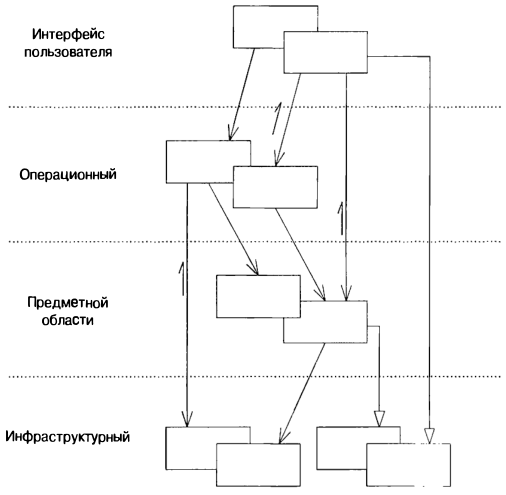
\includegraphics[height=0.8\textheight]{layers.png}
		\end{center}
	\end{frame}

	\begin{frame}
		\frametitle{Изоляция предметной области, соображения}
		\begin{itemize}
			\item Модель предметной области должна быть отделена от остальной программы
			\item Классы модели умеют делать только ``суть''
			\item Сборка всего воедино и общее управление процессом --- на операционный уровень
			\begin{itemize}
				\item Бизнес-регламенты --- на уровне модели предметной области
			\end{itemize}
			\item Все технические вещи --- на инфраструктурный уровень
			\begin{itemize}
				\item Работа с БД
				\item Middleware, сетевые коммуникации
				\item Утилиты
				\item Абстрактные базовые классы
			\end{itemize}
			\item Observer или вариации MVC для связей ``снизу вверх''
		\end{itemize}
	\end{frame}

	\begin{frame}
		\frametitle{Антипаттерн ``Умный GUI''}
		\begin{itemize}
			\item А давайте всю бизнес-логику писать прямо в обработчиках на форме
			\item Код GUI напрямую работает с БД
			\item Делает невозможным проектирование по модели
			\item Не всегда плохо
			\begin{itemize}
				\item Применимы средства быстрой разработки приложений
				\item Прирост производительности на начальных этапах
				\item Легко приделывать новые фичи и переписывать старые
			\end{itemize}
			\item Не всегда хорошо
			\begin{itemize}
				\item Очень сложно переиспользование
				\item Сложно реализовать сложное поведение (зато легко простое)
				\item Сложно интегрироваться
			\end{itemize}
		\end{itemize}
	\end{frame}

	\begin{frame}
		\frametitle{Основные структурные элементы модели}
		\begin{itemize}
			\item \textbf{Ассоциации} --- чем проще, тем лучше
			\item \textbf{Сущность (Entity)} --- объект, обладающий собственной идентичностью
			\begin{itemize}
				\item Нужна операция идентификации
				\item Нужен способ поддержания идентичности
			\end{itemize}
			\item \textbf{Объект-значение (Value object)} --- объект, полностью определяемый своими атрибутами
			\begin{itemize}
				\item ``Лучше'', чем сущность
				\item Как правило, немутабельны
				\item Могут быть разделяемыми
			\end{itemize}
			\item \textbf{Служба (Service)} --- объект, представляющий операцию
			\begin{itemize}
				\item Как правило, не имеет собственного состояния
				\item Операции нет естественного места в других классах модели
			\end{itemize}
			\item \textbf{Модуль (Module)} --- смысловые части модели
		\end{itemize}
	\end{frame}

	\begin{frame}
		\frametitle{Жизненный цикл объекта}
		\begin{center}
			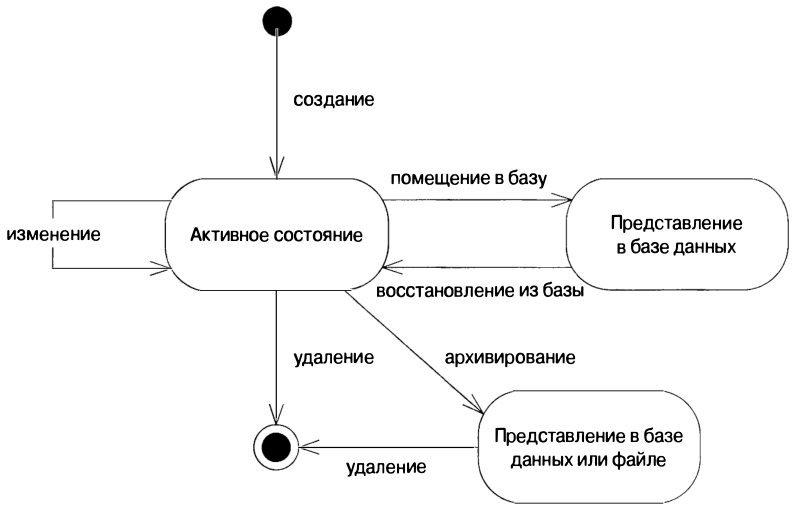
\includegraphics[height=0.7\textheight]{objectLifeCycle.png}
		\end{center}
	\end{frame}

	\begin{frame}
		\frametitle{Агрегаты}
		\begin{itemize}
			\item \textbf{Агрегат} --- изолированный кусок модели, имеющий \textbf{корень} и \textbf{границу}
			\item Корень --- глобально идентичный объект-сущность
			\item Остальные объекты в агрегате идентичны локально
			\item Извне агрегата можно хранить ссылку только на корень
			\begin{itemize}
				\item Отдавать временную ссылку можно
			\end{itemize}
			\item Корень отвечает за поддержание инвариантов всего агрегата
		\end{itemize}
	\end{frame}

	\begin{frame}
		\frametitle{Агрегат, пример}
		\begin{center}
			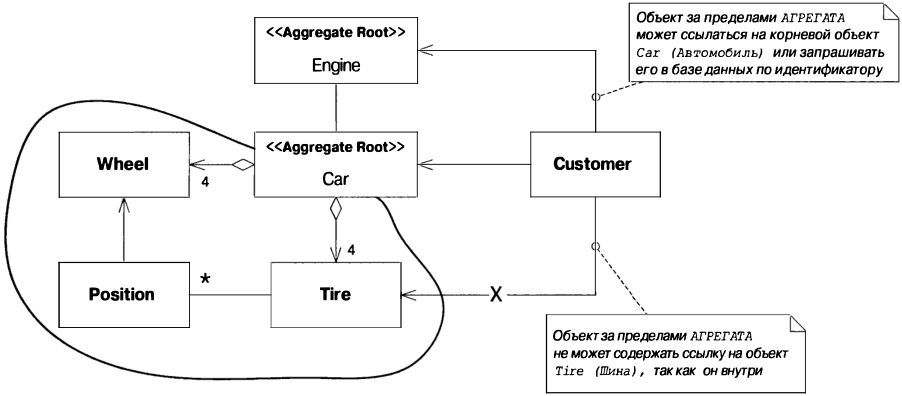
\includegraphics[width=0.9\textwidth]{aggregate.png}
		\end{center}
	\end{frame}

	\begin{frame}
		\frametitle{Агрегат, инварианты}
		\begin{center}
			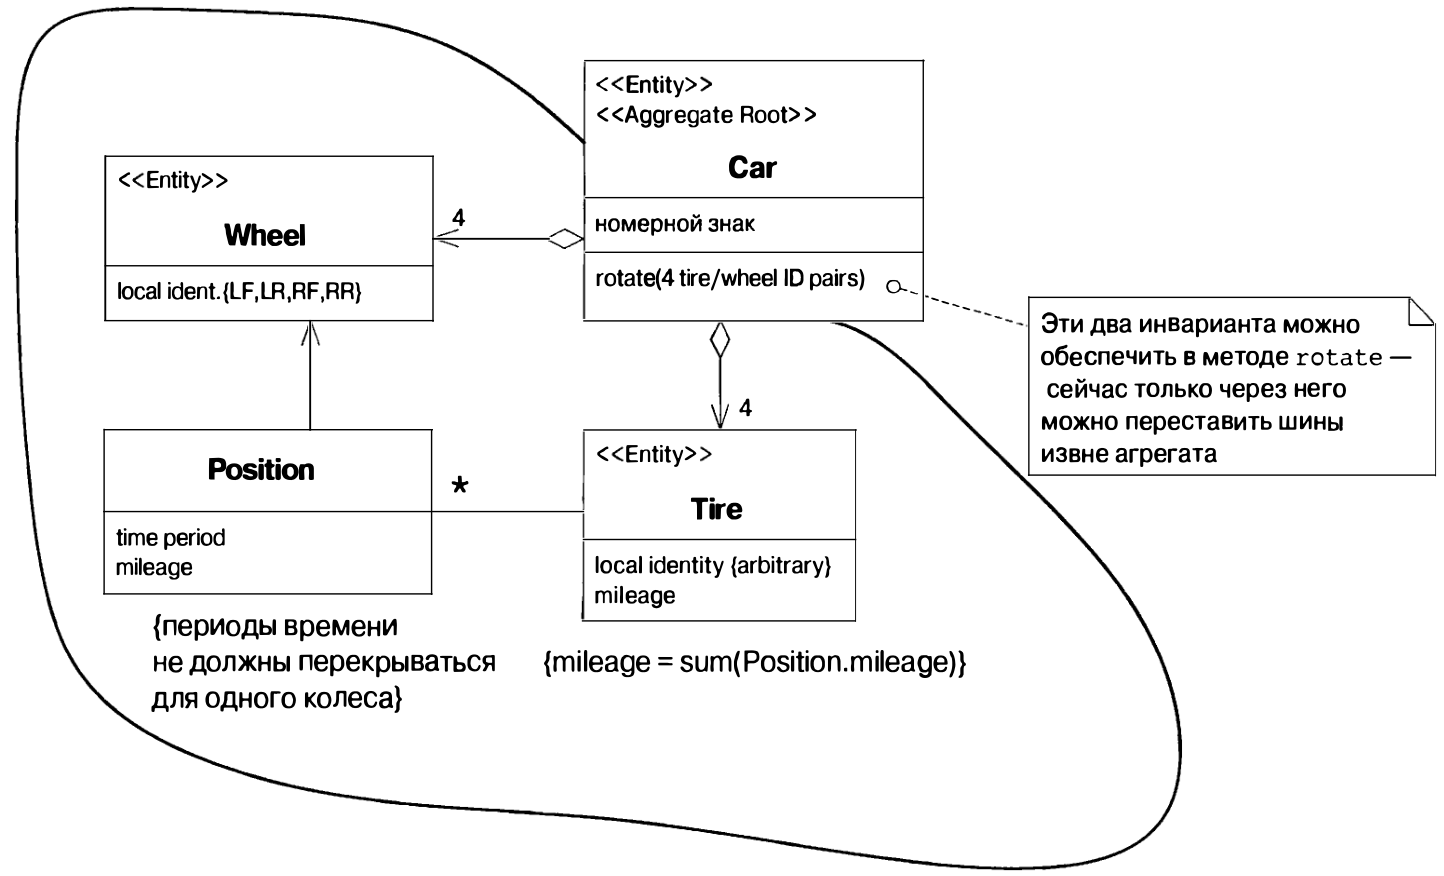
\includegraphics[width=0.9\textwidth]{aggregateInvariants.png}
		\end{center}
	\end{frame}

	\begin{frame}
		\frametitle{Фабрика}
		\begin{center}
			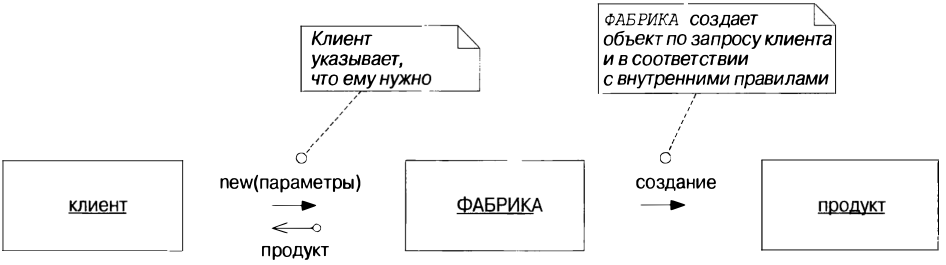
\includegraphics[width=0.7\textwidth]{factory.png}
		\end{center}
		\textbf{Фабрика} служит для создания объектов или агрегатов
		\begin{itemize}
			\item Скрывает внутреннее устройство конструируемого объекта
			\begin{itemize}
				\item Операция создания ``атомарна'' и обеспечивает инварианты
			\end{itemize}
			\item Изолирует сложную операцию создания
			\item Как правило, не имеет бизнес-смысла, но является частью модели
			\item Реализуется аж несколькими разными паттернами
		\end{itemize}
	\end{frame}

	\begin{frame}
		\frametitle{Пример}
		\framesubtitle{Фабрика, использующаяся для восстановления объекта}
		\begin{center}
			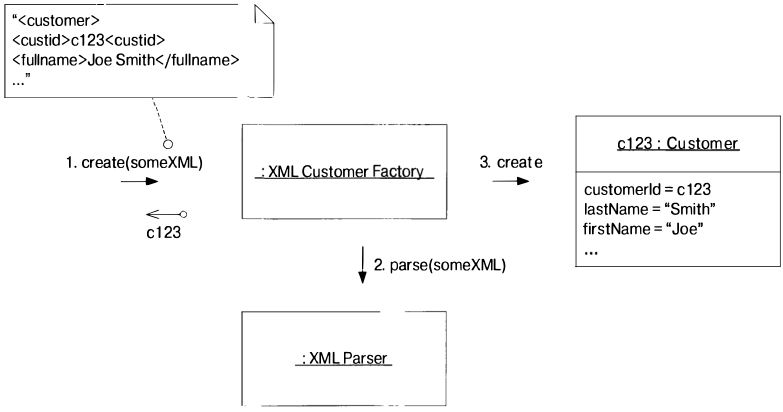
\includegraphics[width=0.8\textwidth]{xmlFactory.png}
		\end{center}
	\end{frame}

	\begin{frame}
		\frametitle{Хранилище (Repository)}
		\begin{center}
			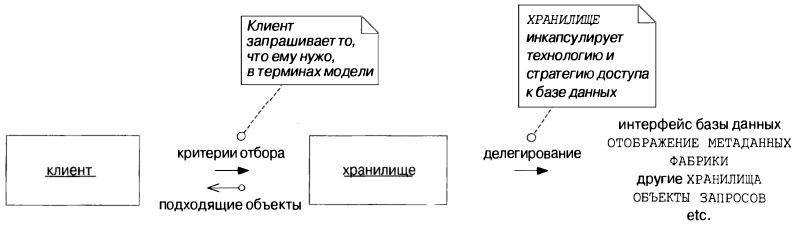
\includegraphics[width=0.8\textwidth]{repository.png}
		\end{center}
		\textbf{Репозиторий} хранит объекты и предоставляет к ним доступ
		\begin{itemize}
			\item Может инкапсулировать запросы к БД
			\item Может использовать фабрики
			\item Может обладать развитым интерфейсом запросов
		\end{itemize}
	\end{frame}

	\section{Пример: система грузоперевозок}

	\begin{frame}
		\frametitle{Пример, система грузоперевозок}
		Требования:
		\begin{enumerate}
			\item Отслеживать ключевые манипуляции с грузом клиента
			\item Оформлять заказ заранее
			\item Автоматически высылать клиенту счет-фактуру по достижении грузом некоторого операционного пункта маршрута
		\end{enumerate}

		\begin{itemize}
			\item В работе с Грузом (Cargo) участвует несколько Клиентов (Customers), каждый из которых играет свою роль (Role)
			\item Должна задаваться (bе specified) цель (goal) доставки груза
			\item Цель (goal) доставки груза достигается в результате последовательности Переездов (Carrier Movement), которые удовлeтворяют Заданию (Specification)
		\end{itemize}
	\end{frame}

	\begin{frame}
		\frametitle{Модель}
		\begin{center}
			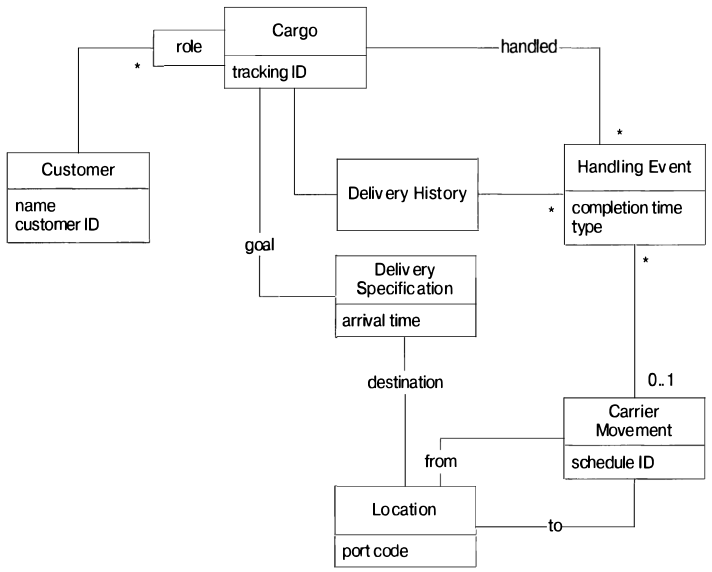
\includegraphics[width=0.7\textwidth]{cargoModel.png}
		\end{center}
	\end{frame}

	\begin{frame}
		\frametitle{Уровень приложения}
		Применим уровневую архитектуру и выделим операции уровня приложения:
		\begin{itemize}
			\item Мaршрутный запрос (Tracking Query) --- манипуляции с конкретным грузом
			\item Служба резервирования (Booking Application) --- позволяет заказать доставку нового груза
			\item Служба регистрации событий (Incident Logging Application) --- регистрирует действия с грузом (связана с маршрутным запросом)
		\end{itemize}
	\end{frame}

	\begin{frame}
		\frametitle{Сущности или значения?}
		\begin{itemize}
			\item \textbf{Клиент (Customer)} --- сущность
			\item \textbf{Груз (Cargo)} --- сущность
			\item \textbf{Манипуляция (Handling Event)} и \textbf{Переезд (Carrier Movement)} --- сущности
			\item \textbf{Местоположение (Location)} --- сущность
			\item \textbf{История доставки (Delivery History)} --- сущность, локально идентична в пределах агрегата ``Груз''
			\item \textbf{Задание на доставку (Delivery Specification)} --- значение
			\item Всё остальное --- значения
		\end{itemize}
	\end{frame}

	\begin{frame}
		\frametitle{Направленность ассоциаций}
		\begin{center}
			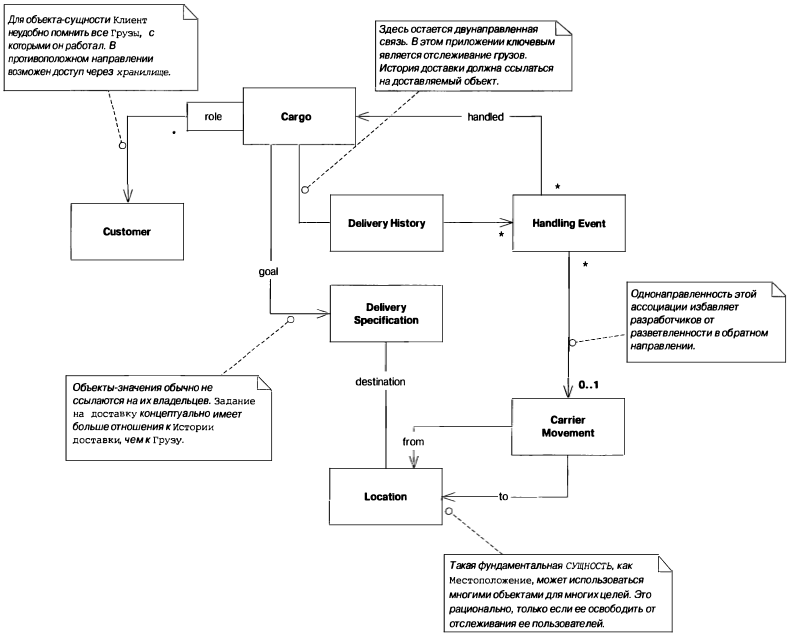
\includegraphics[width=0.8\textwidth]{cargoAssociations.png}
		\end{center}
	\end{frame}

	\begin{frame}
		\frametitle{Границы агрегатов}
		\begin{center}
			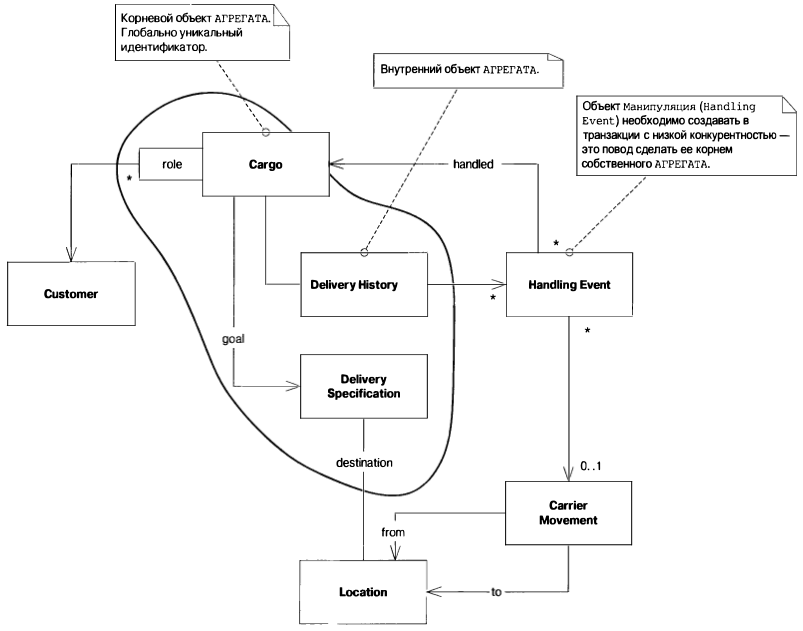
\includegraphics[width=0.82\textwidth]{cargoAggregates.png}
		\end{center}
	\end{frame}

	\begin{frame}
		\frametitle{Хранилища}
		\begin{center}
			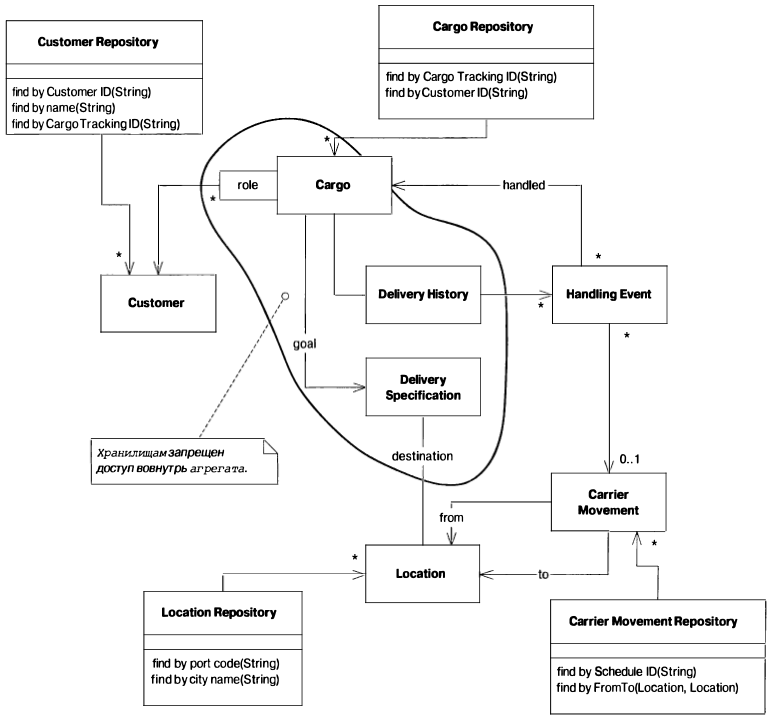
\includegraphics[width=0.69\textwidth]{cargoRepositories.png}
		\end{center}
	\end{frame}

	\begin{frame}
		\frametitle{Тестовый сценарий, добавление события}
		\begin{center}
			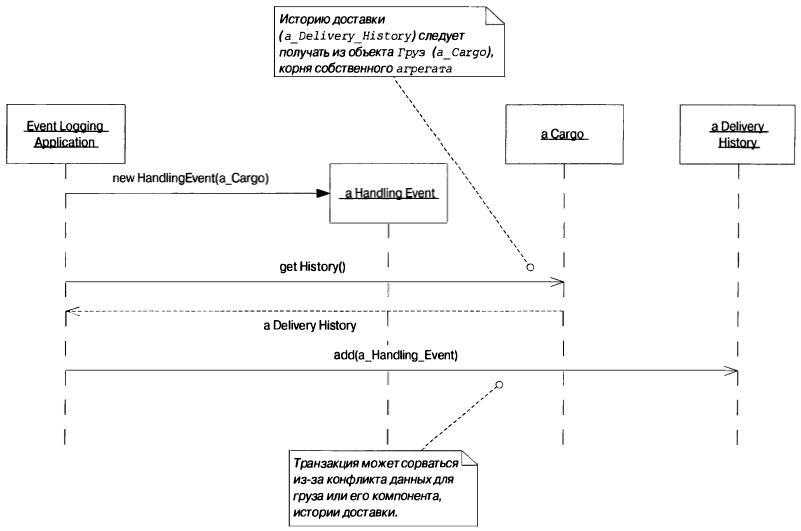
\includegraphics[width=0.8\textwidth]{cargoAddEvent.png}
		\end{center}
	\end{frame}

	\begin{frame}
		\frametitle{Рефакторинг, не хранить события явно}
		\begin{center}
			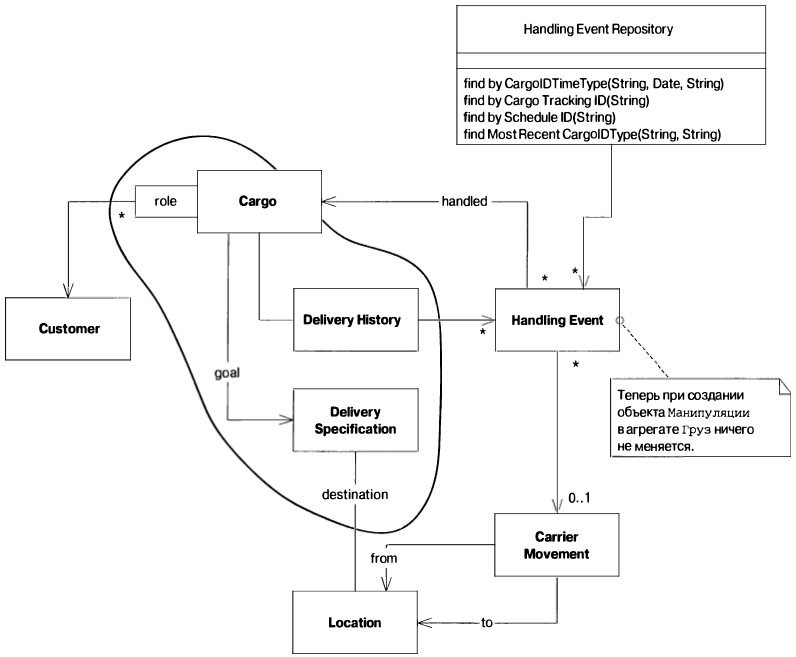
\includegraphics[width=0.7\textwidth]{cargoRefactored.png}
		\end{center}
	\end{frame}

	\begin{frame}
		\frametitle{Разбиение по модулям, плохо}
		\begin{center}
			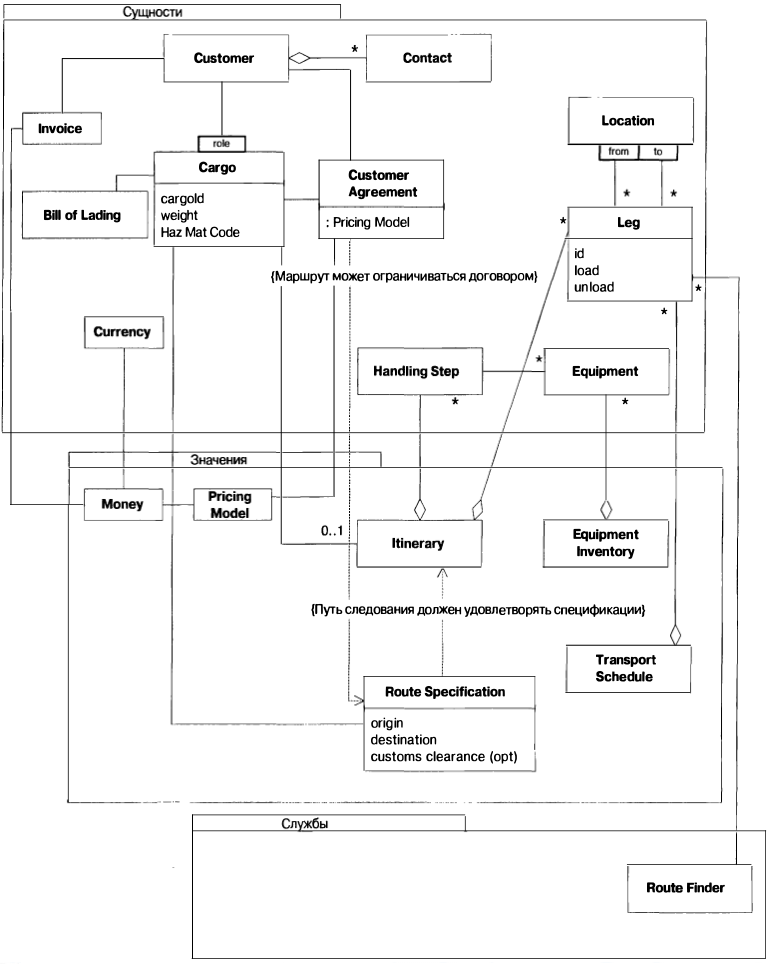
\includegraphics[height=0.9\textheight]{cargoModulesBad.png}
		\end{center}
	\end{frame}

	\begin{frame}
		\frametitle{Разбиение по модулям, хорошо}
		\begin{center}
			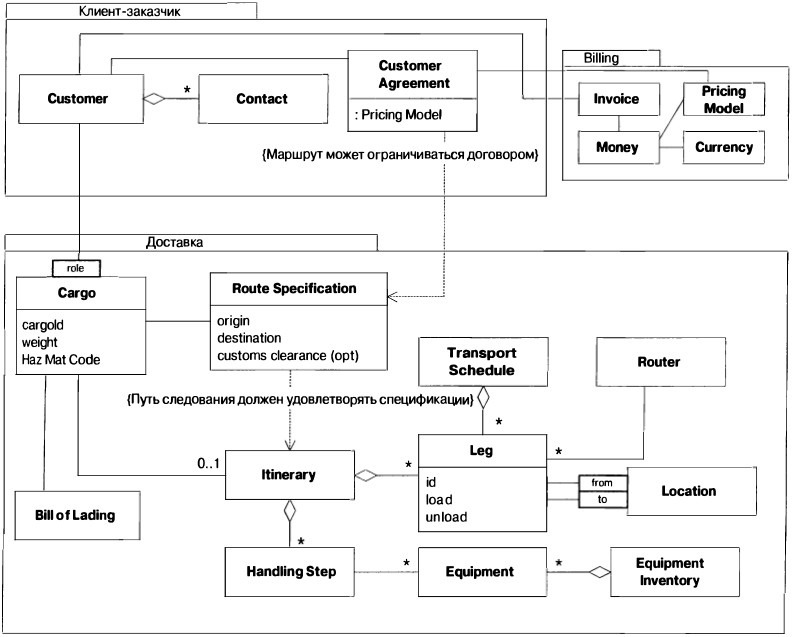
\includegraphics[height=0.8\textheight]{cargoModulesGood.png}
		\end{center}
	\end{frame}

	\section{Моделирование ограничений}

	\begin{frame}
		\frametitle{Моделирование ограничений}
		\framesubtitle{Простой пример}
		\begin{center}
			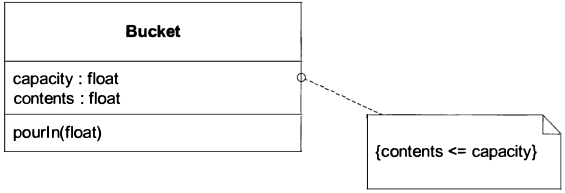
\includegraphics[width=0.6\textwidth]{bucket.png}
		\end{center}
	\end{frame}

	\begin{frame}[fragile]
		\frametitle{Код, до}
		\begin{minted}{java}
class Bucket {
    private float capacity;
    private float contents;

    public void pourIn(float addedVolume) {
        if (contents + addedVolume > capacity) {
            contents = capacity;
        } else {
            contents = contents + addedVolume;
    }
}
		\end{minted}
	\end{frame}

	\begin{frame}[fragile]
		\frametitle{Код, после}
		\begin{minted}{java}
class Bucket {
    private float capacity;
    private float contents;

    public void pourIn(float addedVolume) {
        float volumePresent = contents + addedVolume;
        contents = constrainedToCapacity(volumePresent);
    }

    private float constrainedToCapacity(float volumePlacedIn) {
        if (volumePlacedIn > capacity) return capacity;
        return volumePlacedIn;
    }
} 
		\end{minted}
	\end{frame}

	\begin{frame}
		\frametitle{Паттерн ``Спецификация''}
		\begin{center}
			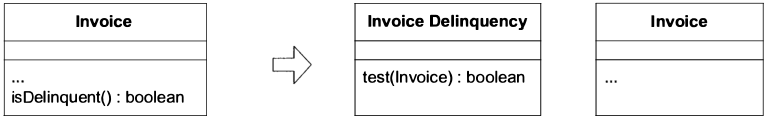
\includegraphics[width=0.8\textwidth]{specification.png}
		\end{center}
		\textbf{Спецификация} инкапсулирует ограничение в отдельном объекте
		\begin{itemize}
			\item Предикат
			\item Может быть использована для выборки или конструирования объектов
		\end{itemize}
	\end{frame}

	\begin{frame}
		\frametitle{Композитные спецификации}
		\begin{center}
			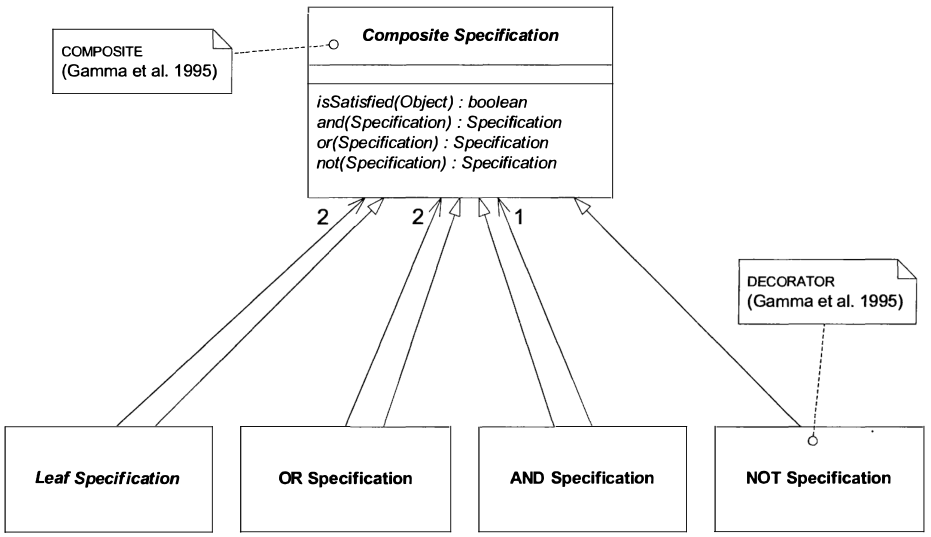
\includegraphics[height=0.7\textheight]{compositeSpecifications.png}
		\end{center}
	\end{frame}

	\begin{frame}
		\frametitle{Пример: склад химикатов}
		\begin{center}
			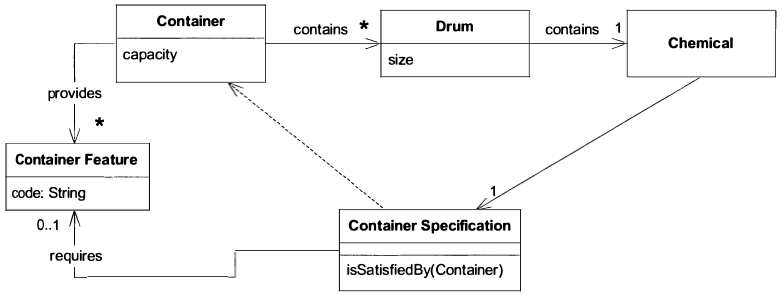
\includegraphics[width=0.9\textwidth]{chemicalsStructure.png}
		\end{center}
	\end{frame}

	\begin{frame}[fragile]
		\frametitle{Код, спецификация}
		\begin{minted}{java}
public class ContainerSpecification {
    private ContainerFeature requiredFeature;

    public ContainerSpecification(ContainerFeature required) {
        requiredFeature = required;
    }

    boolean isSatisfiedBy(Container aContainer) {
        return aContainer.getFeatures().contains(requiredFeature);
    }
}
		\end{minted}
	\end{frame}

	\begin{frame}[fragile]
		\frametitle{Код, контейнер}
		\begin{minted}{java}
boolean isSafelyPacked() {
    Iterator it = contents.iterator();
    while (it.hasNext()) {
        Drum drum = (Drum) it.next() ;
        if (!drum.containerSpecification().isSatisfiedBy(this))
            return false ;
    }
    return true;
}
		\end{minted}
	\end{frame}

	\section{Гибкая архитектура}

	\begin{frame}[fragile]
		\frametitle{Пример рефакторинга, смешивание красок}
		\framesubtitle{Начальное состояние}
		\begin{center}
			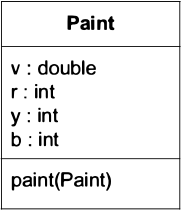
\includegraphics[height=0.3\textheight]{originalPaint.png}
		\end{center}
		\begin{footnotesize}
			\begin{minted}{java}
public void paint (Paint paint) {
    v = v + paint.getV();  // После смешивания объем суммируется
// Опущено много строк сложного расчета смешивания цветов,
// который заканчивается присваиванием новых значений
// компонентов r (красного), b (синего) и y (желтого).
}
			\end{minted}
		\end{footnotesize}
\end{frame}

	\begin{frame}[fragile]
		\frametitle{Шаг 1: говорящий интерфейс}
		\begin{center}
			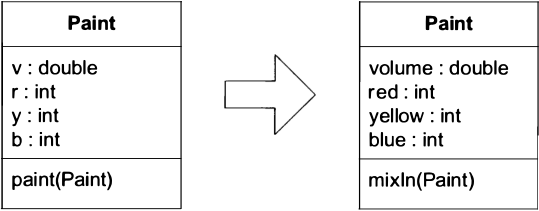
\includegraphics[width=0.4\textwidth]{informativeInterfaceForPaint.png}
		\end{center}
		\begin{footnotesize}
			\begin{minted}{java}
public void testPaint() {
    // Начинаем с чистой желтой краски объемом = 100
    Paint ourPaint = new Paint(100.0, 0, 50, 0);
    // Берем чистую синюю краску объемом = 100
    Paint bluе = new Paint(100.0, 0, 0, 50);
    // Примешиваем синюю краску к желтой
    ourPaint.mixIn(blue); 
    // Должно получиться 200.0 единиц зеленой краски
    assertEquals(200.0, ourPaint.getVolume(), 0.01);
    assertEquals(25, ourPaint.getBlue());
    assertEquals(25, ourPaint.getYellow());
    assertEquals(0, ourPaint.getRed());
}
			\end{minted}
		\end{footnotesize}
\end{frame}

	\begin{frame}
		\frametitle{Шаг 2: функции без побочных эффектов (1)}
		\framesubtitle{Проблема}
		\begin{center}
			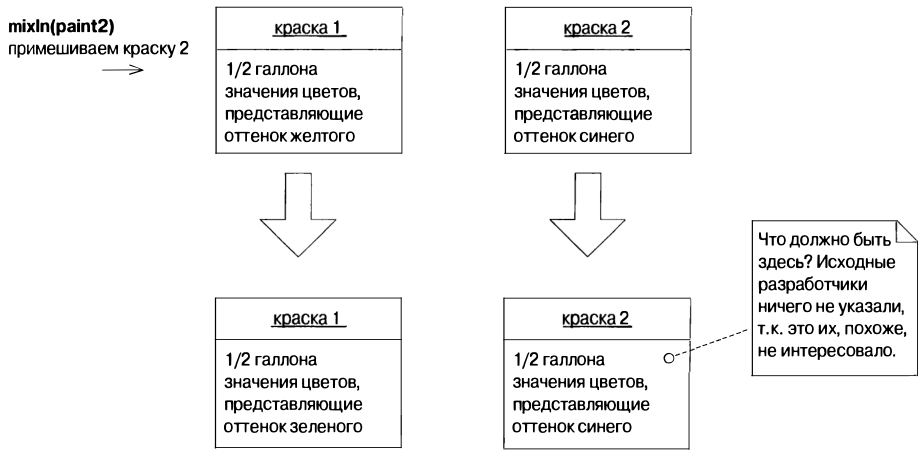
\includegraphics[width=0.9\textwidth]{mixinSideEffects.png}
		\end{center}
	\end{frame}

	\begin{frame}
		\frametitle{Шаг 2: функции без побочных эффектов (2)}
		\framesubtitle{Идея рефакторинга}
		\begin{center}
			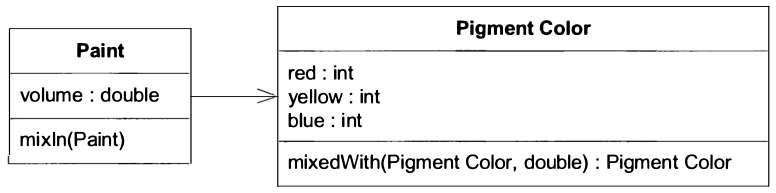
\includegraphics[width=0.8\textwidth]{pigmentColor.png}
		\end{center}
	\end{frame}

	\begin{frame}[fragile]
		\frametitle{Шаг 2: функции без побочных эффектов (3)}
		\framesubtitle{Рефакторинг}
		\begin{footnotesize}
			\begin{minted}{java}
public class PigmentColor {
    public PigmentColor mixedWith(PigmentColor other, double ratio) {
        // Много строк сложного расчета смешивания цветов.
        // в результате создается новый объект PigmentColor
        // с новыми пропорциями красного, синего и желтого.
    }
}

public class Paint {
    public void mixIn(Paint other) {
        volume = volume + other.getVolume();
        double ratio = other.getVolume() / volume;
        pigmentColor = pigmentColor.mixedWith(other.pigmentColor(), ratio);
    }
}
			\end{minted}
		\end{footnotesize}
\end{frame}

	\begin{frame}
		\frametitle{Шаг 2: функции без побочных эффектов (4)}
		\framesubtitle{Результат}
		\begin{center}
			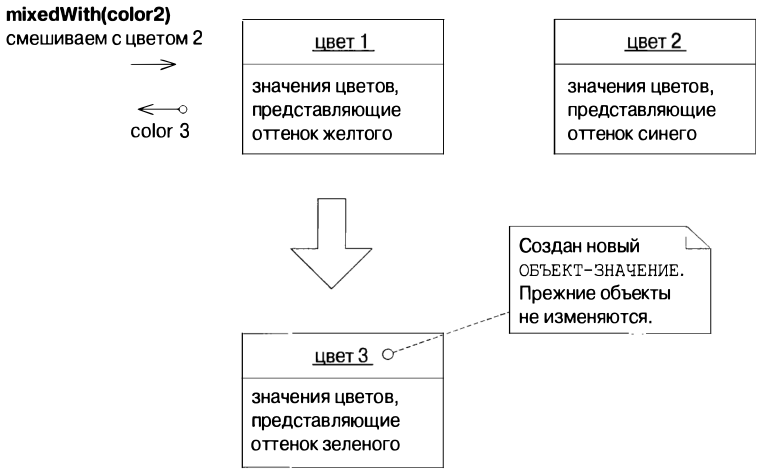
\includegraphics[width=0.8\textwidth]{pigmentColorValueObject.png}
		\end{center}
	\end{frame}

	\begin{frame}[fragile]
		\frametitle{Шаг 3: assertions (1)}
		\framesubtitle{Инварианты, как они есть}
		Постусловие для mixIn():
		{\color{blue}
		\begin{verbatim}
После pl.mixIn(p2):
    pl.volume увеличивается на объем p2.volume
    p2.volume не изменяется
\end{verbatim} }
		И инвариант:
		{\color{blue}
		\begin{verbatim}
Общий объем краски не должен измениться от смешивания
\end{verbatim} }
	???
\end{frame}

	\begin{frame}
		\frametitle{Шаг 3: assertions (2)}
		\framesubtitle{Рефакторинг}
		\begin{center}
			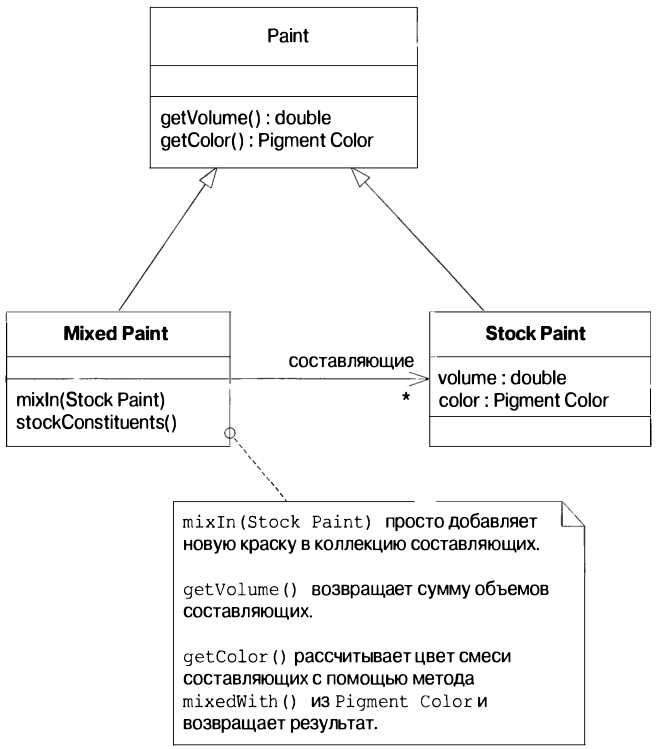
\includegraphics[height=0.8\textheight]{stockPaints.png}
		\end{center}
	\end{frame}

	\section{Задача: Roguelike}

	\begin{frame}
		\frametitle{Домашнее задание: Roguelike}
		\begin{itemize}
			\item Жанр компьютерных игр, назван в честь игры Rogue, 1980 года выхода
			\item Характеризуется:
			\begin{itemize}
				\item Простой тайловой или консольной графикой
				\item Активным использованием случайной генерации
				\item Перманентной смертью персонажа и невозможностью загрузить предыдущее сохранение
				\item Чрезвычайно развитым набором игровых правил
				\item Высокой свободой действий персонажа (``игры-песочницы'')
			\end{itemize}
			\item Примеры:
			\begin{itemize}
				\item \url{https://en.wikipedia.org/wiki/NetHack}
				\item \url{https://en.wikipedia.org/wiki/Angband_(video_game)}
				\item \url{https://en.wikipedia.org/wiki/Ancient_Domains_of_Mystery}
			\end{itemize}
		\end{itemize}
	\end{frame}

	\begin{frame}
		\frametitle{Что хочется}
		\begin{itemize}
			\item Персонаж игрока, способный перемещаться по карте, управляемый с клавиатуры
			\begin{itemize}
				\item Непосредственно стрелками (или дополнительной цифровой клавиатурой), не вводом команды
			\end{itemize}
			\item Инвентарь персонажа, включающий элементы, влияющие на его характеристики, которые можно надеть и снять
			\item Карта (автоматически сгенерированная или считываемая из файла, на ваше усмотрение)
			\item Мобы, способные перемещаться по карте
			\item Боевая система --- движущиеся объекты, пытающиеся занять одну клетку карты, атакуют друг друга
			\item Все детали --- на ваше усмотрение
		\end{itemize}
	\end{frame}

	\begin{frame}
		\frametitle{Задача 1: Архитектура Roguelike}
		Построить модель предметной области и модель структуры консольной Roguelike RPG
		\begin{itemize}
			\item Модель предметной области не обязательно делать отдельной диаграммой
			\item Ожидаемый результат --- диаграмма компонентов и диаграммы классов для каждого компонента
			\begin{itemize}
				\item Достаточно подробная, чтобы её можно было отдать на реализацию неопытному программисту
			\end{itemize}
			\item Дедлайн: \textbf{10:00 20.04.2018г.}
		\end{itemize}
	\end{frame}

	\begin{frame}
		\frametitle{Задача 2: Roguelike}
		\begin{columns}
			\begin{column}{0.5\textwidth}
				Реализовать Roguelike RPG.

				\begin{itemize}
					\item Консольная графика, с возможностью далее сделать графический тайловый интерфейс
					\item Расширяемая и сопровождаемая архитектура
					\item Логирование основных событий в игре
					\item Юнит-тесты
				\end{itemize}
				Дедлайн: \textbf{04.05.2018г.}
			\end{column}
			\begin{column}{0.5\textwidth}
				\begin{center}
					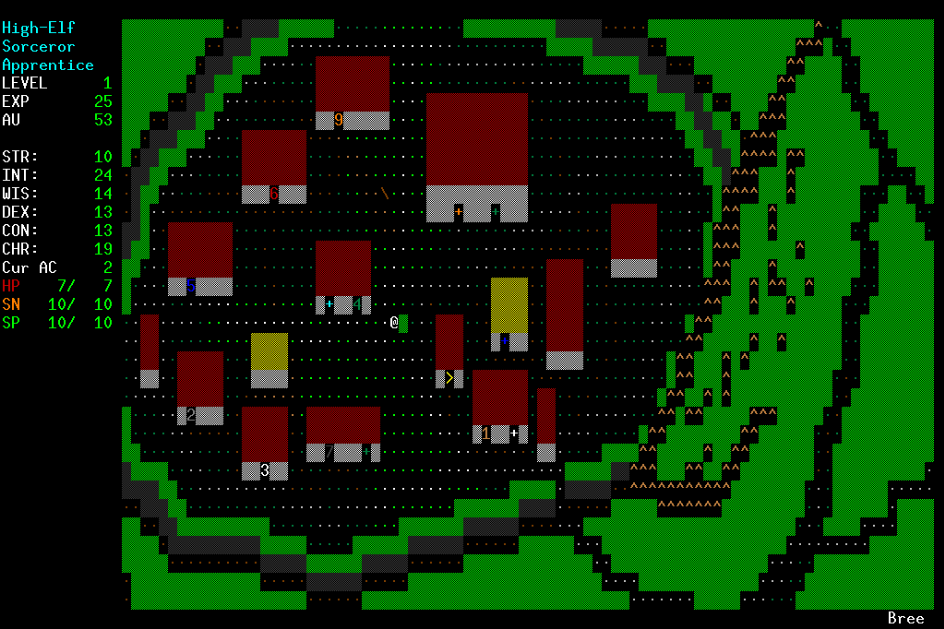
\includegraphics[width=0.9\textwidth]{roguelike.png}
				\end{center}
			\end{column}
		\end{columns}
	\end{frame}

\end{document}
